\section{Data flow}
\label{data_flow_sec}

The data generation and analysis process involves several stages, beginning with sample collection and culminating in the presentation of final results. 
This process is designed to integrate  with existing clinical databases using newly developed OMICs concepts based on the SPHN ontology.
The process is summarised in 
\textbf{figure 
\ref{fig:precision_med_dataflow}.}

We have worked with SPHN and 
\href{https://www.thehyve.nl/articles/bridging-clinical-and-genomics-knowledge}{TheHyve} to develop new concepts which cover the generation of sequencing data and analysis, recently published in \citet{van2023bridging} as illustrated in
\textbf{figure 
\ref{fig:concept}}.
We have also developed the concepts which cover the final outputs of downstream analysis results for omic results.
This work enhances the integration of omics data into the SPHN Semantic Interoperability Framework, which primarily handles clinical routine data. 

Our new genomics extension enriches the framework to include comprehensive descriptions of genomics experiments, encompassing both clinical and research applications. 
It outlines the entire omics process flow, detailing steps from sample processing to data analysis, including specifics like library preparation and sequencing analysis. 
The extension also integrates additional omics metadata, such as details on sequencing instruments and quality control metrics. By aligning with established semantic models and leveraging common biomedical vocabularies (e.g., EDAM, OBI, and FAIR genomes), it promotes semantic interoperability and aims to FAIRify data for shared use within the Swiss network, enhancing data reuse in a unified knowledge graph.

\begin{figure}[h] \hspace*{0cm} 
\begin{center}
	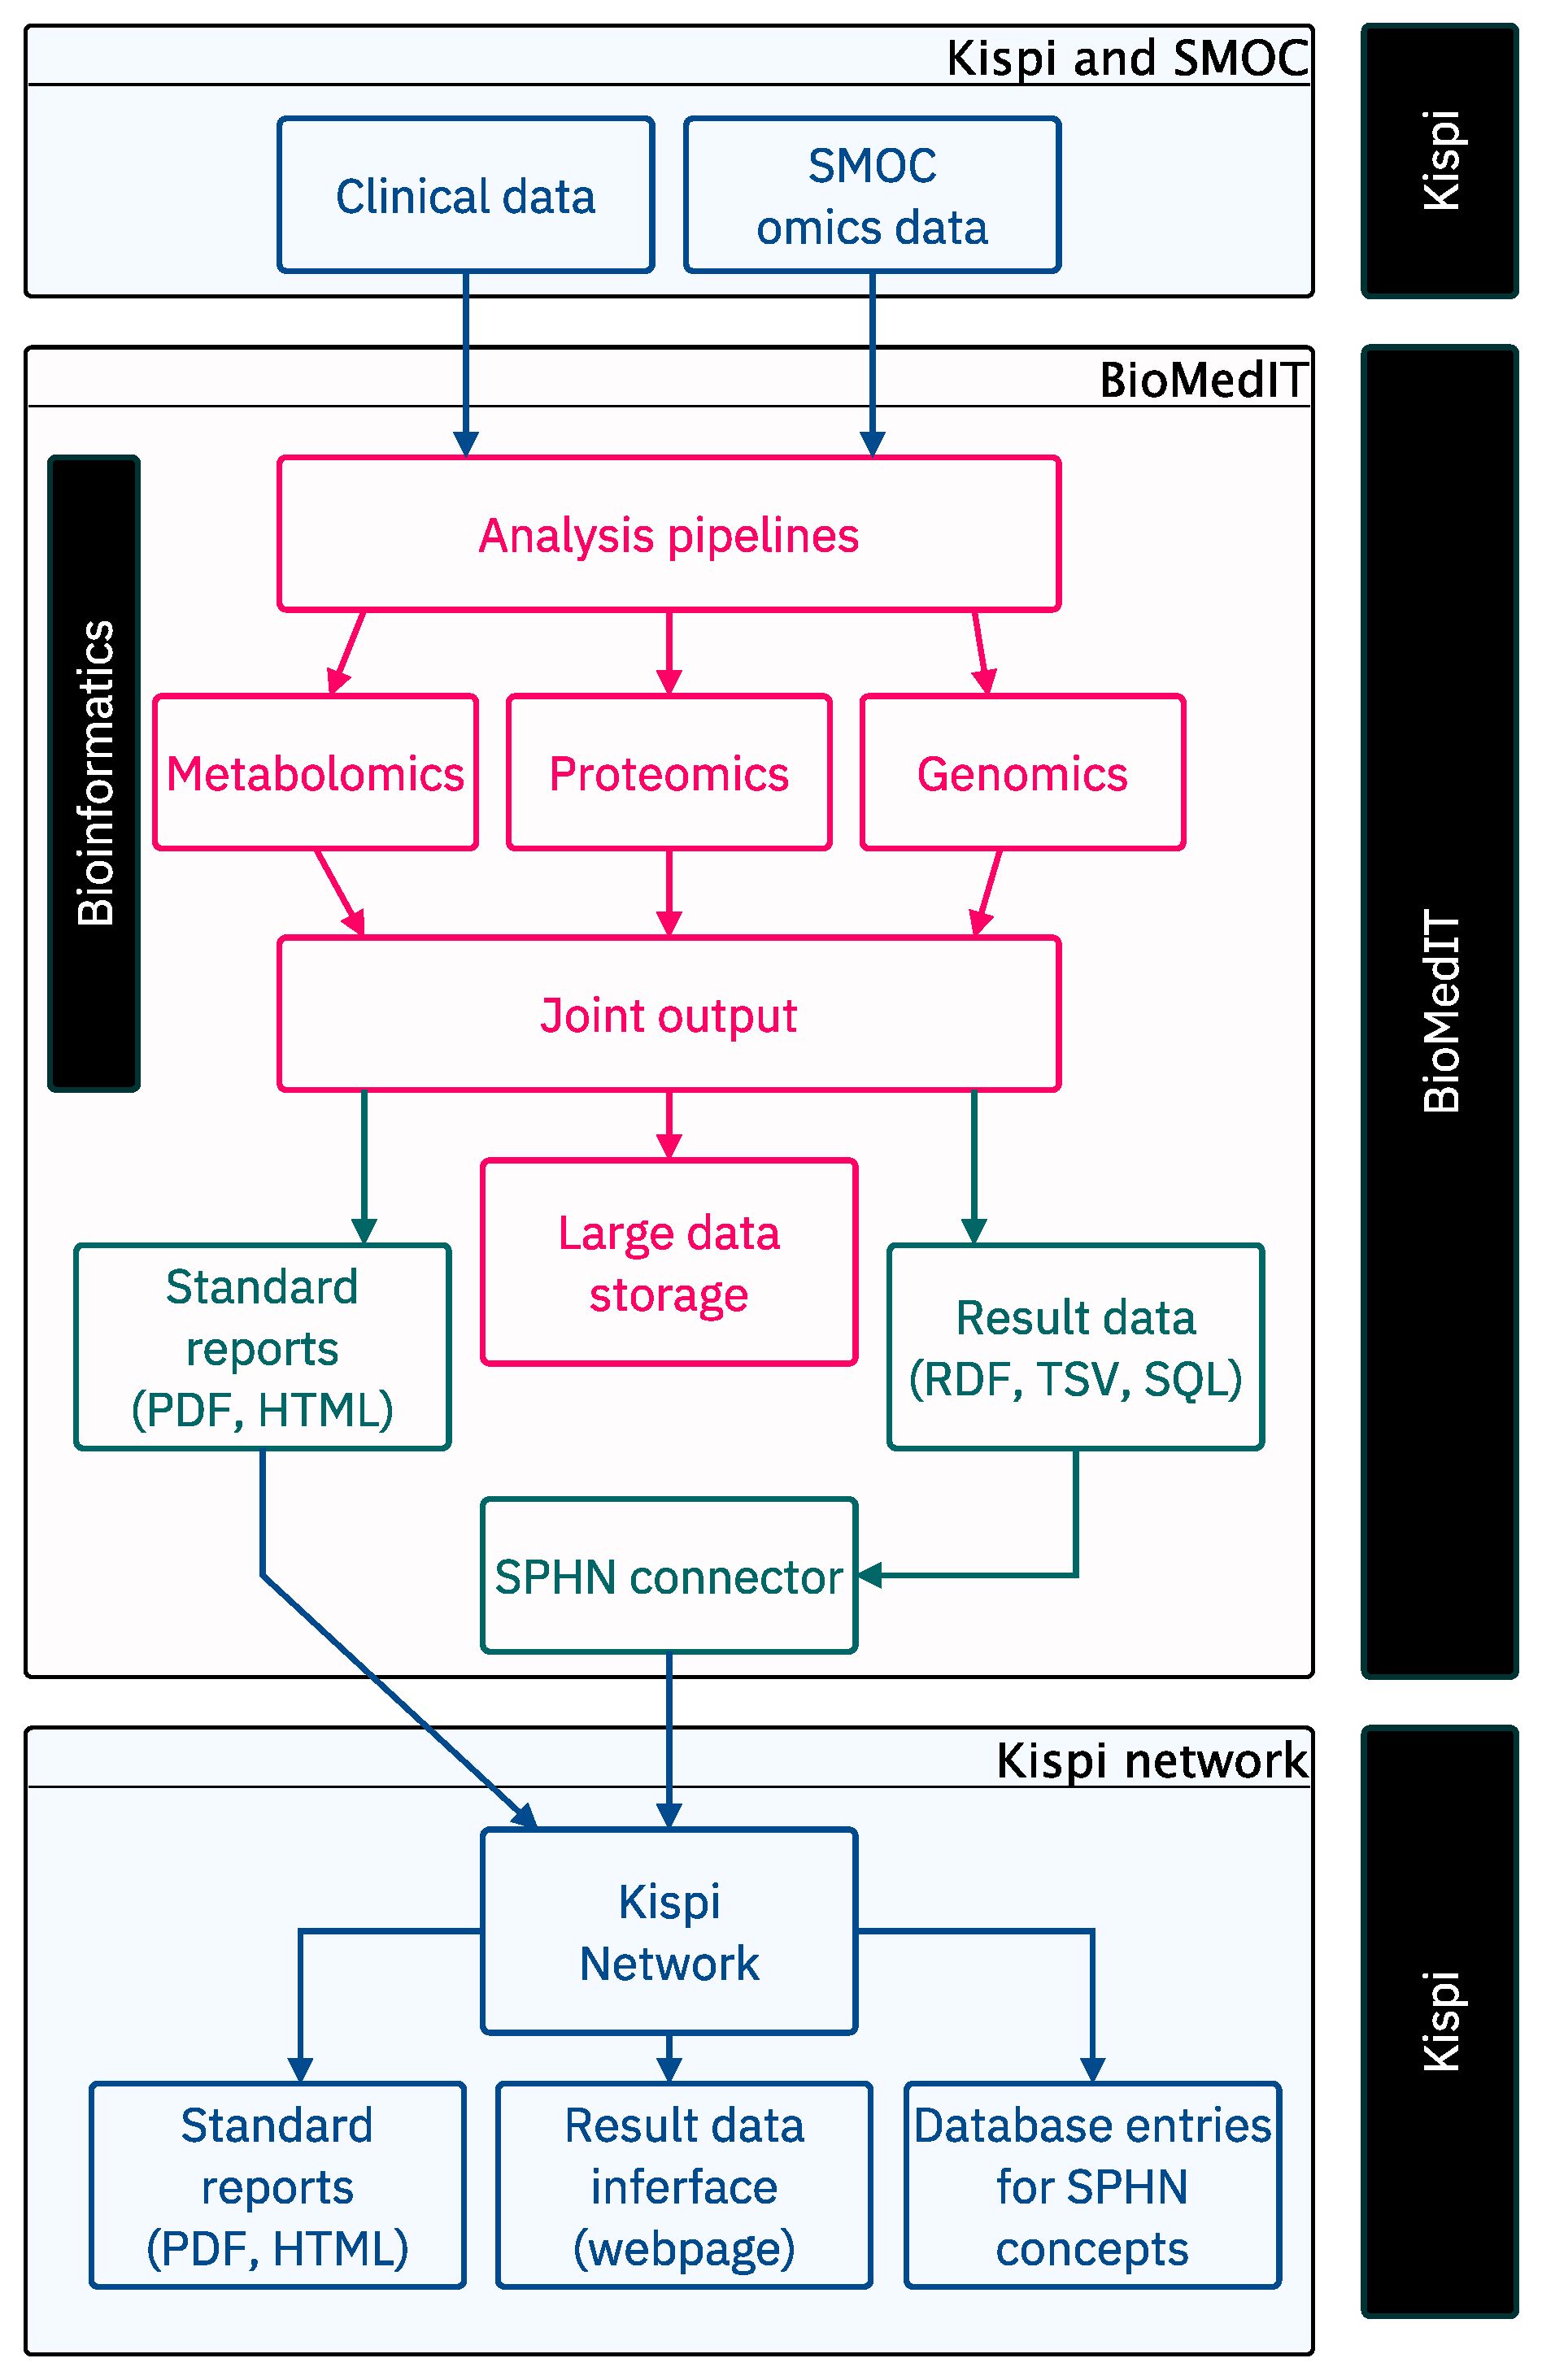
\includegraphics[width=0.6\textwidth]{precision_med_dataflow}
	\caption{\pmu data flow from sample collection to final result presentation. \textbf{Sample collection}: Sample collection occurs in \kispi. SMOC typically processes most physical samples of DNA, RNA, serum, or other tissues. Multi-omic data is generated and transfered to BioMedIT. \textbf{Analysis on BioMedIT}: Bioinformatic analysis pipelines process the data and produce a main analysis output which is stored long-term. 
	Key actionable results from this large dataset are prepared according to SPHN ontology, using concepts such as ``sequencing assay'' and ``omic result''. 
	\textbf{Transfer results to \kispi}:
	Two datasets are prepared before transfer to the \kispi network. (1) The data for which we have SPHN concepts and is suitable for a clinical data warehouse is prepared in TSV, SQL, RDF, or other format. (2) Supplemental reports with extensive metadata, visualisations, and contextual information in formats such as TSV, PDF, HTML. Both datasets are transfered to the \kispi network for database integration and file storage, respectively.}
	\label{fig:precision_med_dataflow}
\end{center}
\end{figure}

\begin{figure}[h] \hspace*{0cm} 
\begin{center}
	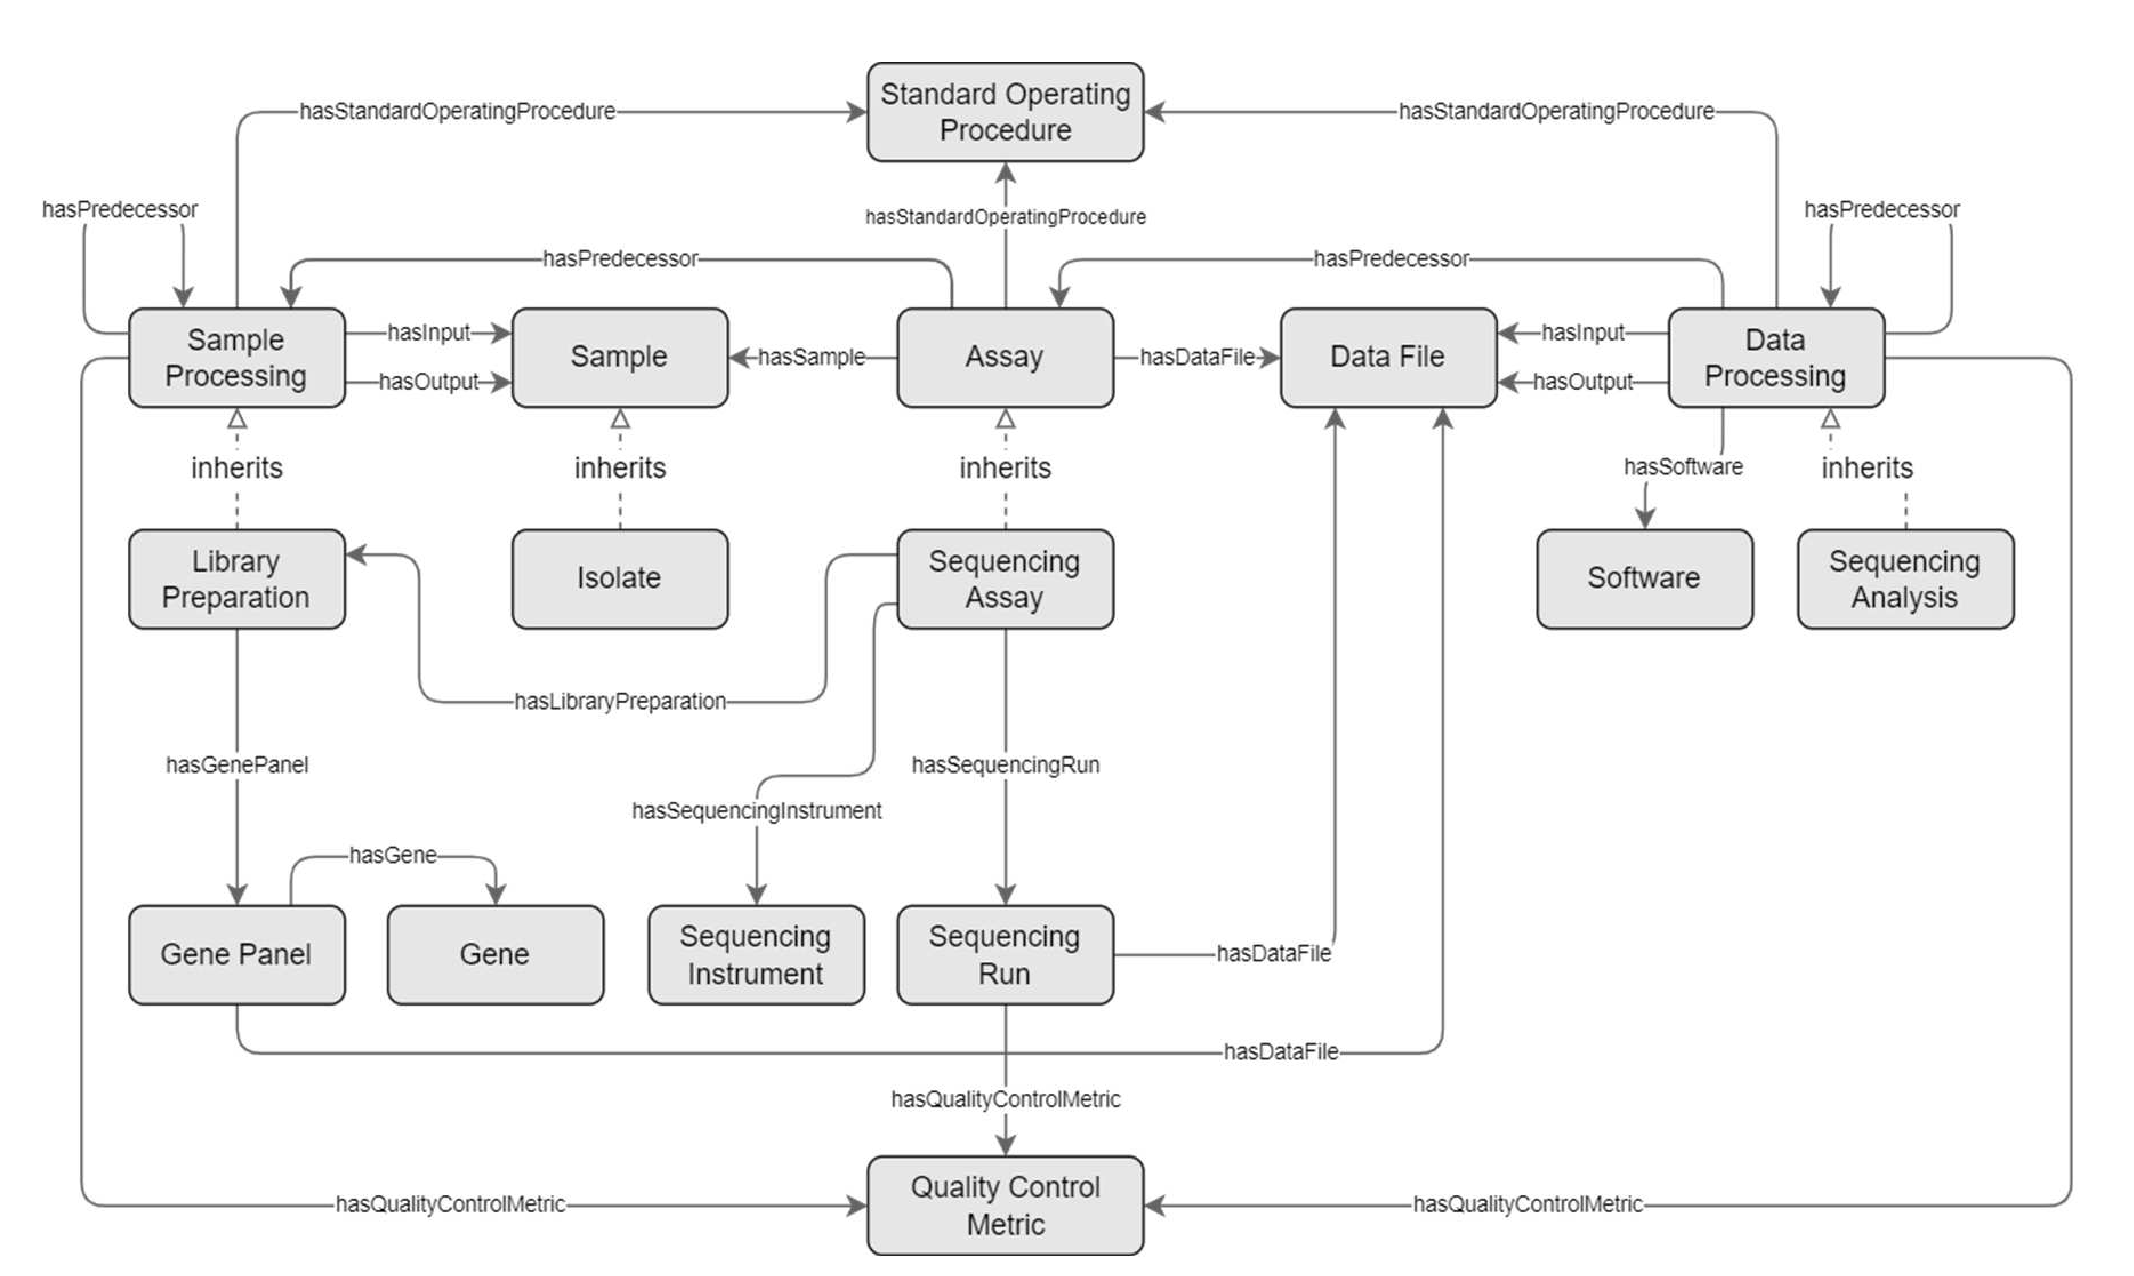
\includegraphics[width=0.8\textwidth]{concept_f1}
	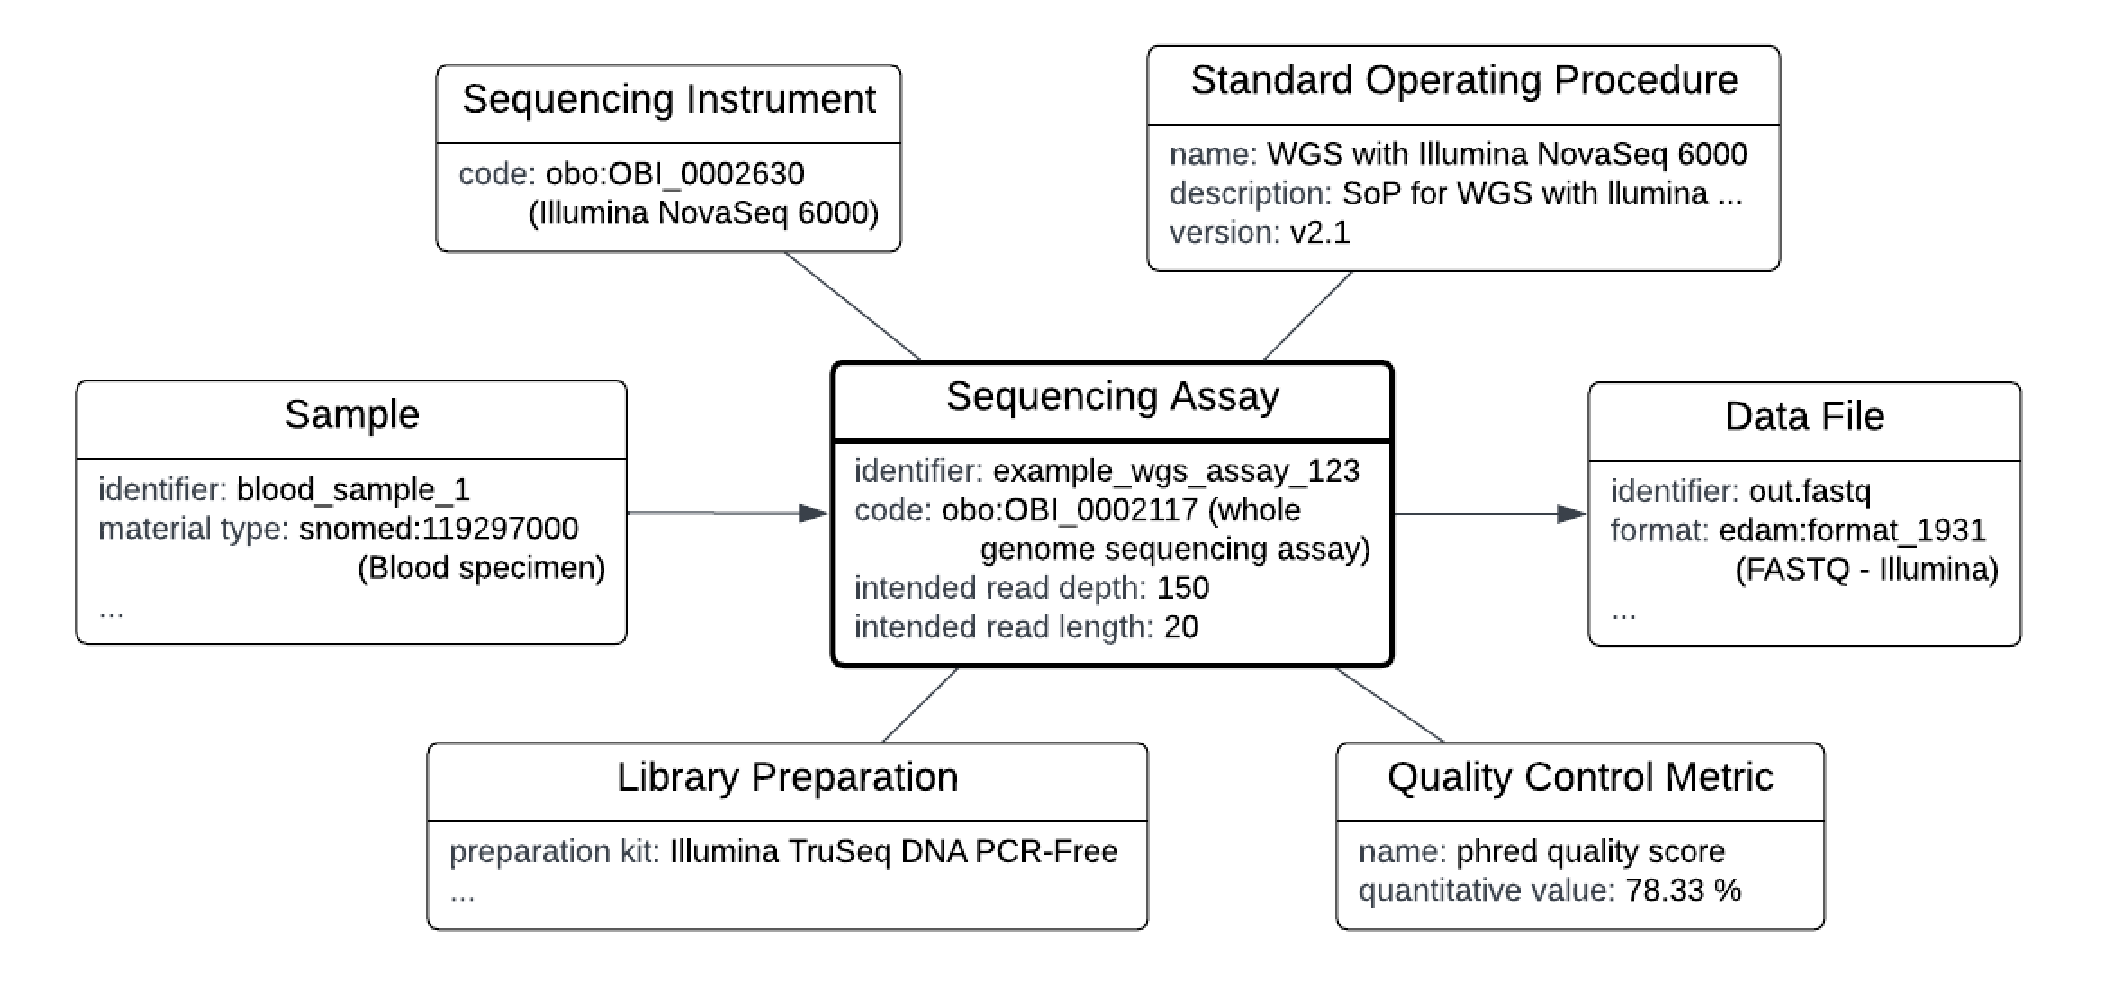
\includegraphics[width=0.8\textwidth]{concept_f2}
	\caption{Figure extract and text quoted from \citet{van2023bridging}: (A) Basic excerpt of the schema for the (gen)omics process flow. (B) Diagram visualising an instance of a sequencing assay that analyses one sample and produces one FASTQ file. ``Sequencing Assay'' concept, together with its ``Instrument'', ``Library Preparation'', ``Standard Operating Procedure'', and ``Quality Control Metric'' concepts from which it is composed.}
	\label{fig:concept}
\end{center}
\end{figure}
\clearpage

\subsection{Sample collection and initial processing}
\begin{itemize}
    \item \textbf{Location:} \kispi.
    \item \textbf{Details:} Sample collection encompasses various biological materials including DNA, RNA, serum, and other tissue types. These are initially processed by the Swiss Multi-Omics Center (SMOC), which is responsible for the physical handling and preliminary omics data generation.
\end{itemize}

\subsection{Data transfer and bioinformatics analysis}
\begin{itemize}
    \item \textbf{Transfer:} The raw multi-omic data generated by SMOC is transferred to BioMedIT using secure protocols such as sFTP.
    \item \textbf{Bioinformatics processing:} At BioMedIT, advanced bioinformatics pipelines are employed to analyse the data. This includes comprehensive analyses across metabolomics, proteomics, and genomics disciplines.
    \item \textbf{Outputs:} The main outputs from these analyses include:
    \begin{itemize}
        \item A large dataset stored for long-term reuse and research purposes.
        \item Standard reports generated in formats such as TSV, PDF, and HTML.
        \item Result data formatted in RDF, SQL, TSV, which are then adapted to meet the SPHN connector’s requirements for merging into clinical data warehouses.
    \end{itemize}
\end{itemize}

\subsection{Data conversion and integration}
\begin{itemize}
    \item \textbf{Conversion:} Key actionable results are extracted from the large dataset and prepared according to our reporting evidence guidelines and formatted using the SPHN ontology. This preparation uses specific OMICS concepts such as ``omic result'' to ensure that the data can be seamlessly integrated and interpreted within the clinical framework.
    \item \textbf{Integration:} The processed results are converted to fit the database requirements of the hospital’s clinical data warehouse.
\end{itemize}

\subsection{Presentation of final results}
\begin{itemize}
    \item \textbf{Internal Network Transfer:} Outputs, including the standard reports and result data, are transferred back to the \kispi network. This step is crucial as clinicians do not have direct access to secured BioMedIT servers.
    \item \textbf{Access and Presentation:} Final analysis results are made accessible to clinicians through an internal webpage and downloadable TSV, PDF, or other formats. This ensures that the results are readily available for clinical decision-making and further research. The clinical data warehouse will maintain the main omic result data in RDF, SQL, or other suitable formats that best match the current system. 
\end{itemize}

By aligning with the SPHN RDF ontology and implementing it through newly developed OMICS concepts, this data flow ensures that genomic and other omic data types are integrated into the hospital’s clinical operations, enhancing the capacity for precision medicine and personalised patient care.
The entire process is illustrated in 
\textbf{figure \ref{fig:precision_med_dataflow}}, 
providing a visual representation of the data flow from sample collection to final result presentation within the hospital’s infrastructure.



